% !TeX spellcheck = nl_NL
\begin{savequote}[0.55\linewidth]
	``Alice: How long is forever? White Rabbit: Sometimes, just one second. —  Alice's Adventures in Wonderland''
	\qauthor{\textasciitilde Lewis Carroll}
\end{savequote}

\chapter{Evaluatie}

\label{chap:onderzoek}
De user-perceived performantie kan afwijken van de werkelijke performantie. Dit verschil wordt voornamelijk bepaald door de interface van de applicatie. Zo ervaren gebruiker wachttijden als minder lang wanneer ze een gevoel van vooruitgang krijgen, door het gebruik van progress bars of andere visuele hints. Aangezien we bij dit onderzoek dezelfde applicatie voor beide API's gebruiken, zullen deze visuele hints de vergelijking van de user perceived performance tussen de twee diensten niet beïnvloeden. Echter biedt Linked Connections de mogelijkheid tot incrementele resultaten: nog tijdens het laden kunnen al snel eerste resultaten weergegeven worden, waardoor de gebruiker deze techniek als sneller kan ervaren, ook al duurt het langer om een gelijk aantal resultaten op te halen. Ook voor LC2Irail zal de applicatie van incrementele resultaten gebruik maken, echter is het hier steeds de server die bepaalt wanneer data verzonden worden. De server zal steeds pogen om een bepaald tijdsinterval te verwerken, of een bepaald aantal resultaten te vinden alvorens de client te antwoorden. Hierdoor kunnen de resultaten wel per tijdsinterval getoond worden, maar niet zo atomair als wanneer Linked Connections gebruikt wordt.

In figuur~\ref{fig:expectedserviceperceivedservice} zien we de factoren die bijdragen tot de verwachting van de gebruiker en de ervaring van de gebruiker. De User Experience wordt hier tot de \foreign{service delivery} gerekend. Naast het verschil tussen de werkelijke geleverde service en de ervaren service, merken we ook een verschil tussen de verwachte service en de ervaren service, in Engelstalige literatuur omschreven als een `service quality gap'. De verwachtte service is wat de gebruiker verwacht van de applicatie, onder andere in termen van snelheid, mogelijkheden en dataverbruik. Dit correleert duidelijk met de User Experience: eerder onderzoek wijst uit dat interface design, prestaties van de applicatie, batterijgebruik, kostprijs van de applicatie en connectiviteit, gebruiksersroutines en levensstijl invloed hebben op de user experience~\citep{ickin12}. In dit onderzoek zullen we ons specifiek richten op de prestaties, batterijverbruik, dataverbruik en  offline beschikbaarheid.

De gebruiker heeft geen exact beeld over batterijverbruik en dataverbruik, maar wel over snelheid en offline beschikbaarheid. Of de gebruiker Linked Connections als snel ervaart, zal indirect bepaald worden door de snelheid van alle andere applicaties die hij gebruikt (past experiences) en de tijd die hij kan wachten op een antwoord (personal needs). Zo vinden we het bijvoorbeeld normaal dat een video uploaden enkele minuten kan duren, terwijl we verwachten dat het verzenden van een chatbericht dat enkel uit tekst bestaat onmiddellijk gaat. In dit geval is de verwachtte service gebaseerd op de bestaande applicaties, welke allemaal ongeveer gelijke prestaties bieden en gebruikmaken van RPC API's. De personal need is om onmiddellijk informatie op te zoeken, zonder veel vertraging. Met andere woorden verwacht de gebruiker om binnen enkele seconden de informatie te krijgen.

\begin{figure}[h]
	\centering
	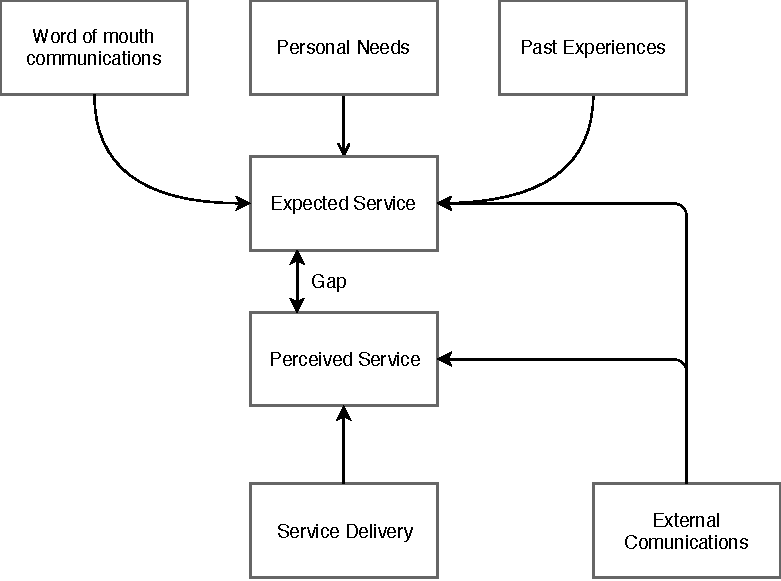
\includegraphics[width=1.00\textwidth]{expected_service.pdf}
	\caption[Factoren die bijdragen tot de verwachtingen van de gebruiker]{Factoren die bijdragen tot de verwachtingen van de gebruiker}
	\label{fig:expectedserviceperceivedservice}
\end{figure}

Tijdens dit onderzoek zullen we zowel de \foreign{service delivery} als \foreign{perceived service} proberen vergelijken tussen de twee technieken. Door deze vergelijking zullen we kunnen vaststellen of Linked Connections een betere user-perceived performance biedt, zowel absoluut als relatief ten opzichte van de werkelijke performance.

Een diepgaand onderzoek over de verwachte service valt buiten het bereik van deze masterproef. We zullen echter wel bondig de verwachtingen van gebruikers ondervragen, op vlak van dataverbruik, offline functionaliteit, en privacy, gezien deze drastisch verschillen bij Linked Connections ten opzichte van meer traditionele API's.

\section{Objectieve metingen}

Met objectieve metingen zullen we de werkelijke performance van elke API vastleggen. Ook zullen we het dataverbruik en batterijverbruik van beide technieken aan de hand van deze metingen trachten te bepalen.

Aangezien het onmogelijk is om automatisch volledige zoekopdrachten uit te voeren door de applicatie zonder de benodigde tijd te beïnvloeden, en aangezien de benodigde tijd om te renderen een constante is die gelijk is voor alle implementaties, zal er rechtstreeks op de API implementatie getest worden, net zoals de API normaal gezien gebruikt wordt. Het uittekenen van de resultaten op het scherm is een constante, welke verwaarloosbaar klein is in vergelijking met de tijd benodigd voor het ophalen van resultaten.

Om te voorkomen dat de keuze van het geteste stations of routes de objectieve metingen vertekent, zullen we de opzoekingen van echte gebruikers gebruiken. Hiervoor gebruiken we de log data van api.irail.be, die publiek beschikbaar zijn\footnote{https://gtfs.irail.be/logs}. Door deze queries opnieuw af te spelen op de applicaties kunnen we een zo goed mogelijk beeld krijgen van de werkelijke prestaties.

Objectief zullen we proberen om volgende gegevens vast te leggen
\begin{itemize}
	\item de gemiddelde tijd om alle data van de server te halen
	\item de gemiddelde tijd tussen zoekopdracht en weergave van het eerste resultaat
	\item de gemiddelde tijd tussen zoekopdracht en weergave van de eerste tien resultaten
	\item de gemiddelde hoeveelheid data die verzonden en ontvangen wordt
	\item het gemiddelde processorgebruik van het toestel
	\item het gemiddelde batterijgebruik van het toestel
\end{itemize}

Hiertoe zullen we gebruik maken van een HTC 10 en een HTC One. Dit zijn twee smartphones in een zeer verschillende klasse op vlak van hardware én software. De verschillen tussen beide toestellen worden verduidelijkt in tabel~\ref{tab:testdevices}
\begin{table}[ht]
	\begin{tabular}{| c | c | c |}
		\hline
		Kenmerk & HTC One M7 & HTC 10 \\
		\hline
		Besturingssysteem & Android 5.0 & Android 8.0 \\
		Processor & Qualcomm Snapdragon 600 & Qualcomm Snapdragon 820\\
		& (4x Krait 1,7GHz) & (4x Kryo 2,2GHz) \\
		Werkgeheugen & 2GB & 4GB \\
		Wi-Fi & 802.11ac & 802.11ac \\
		\hline
		Antutu Benchmark & 31.447 (mediaan)  & 133.791 (top 10\%) \\
		\hline
	\end{tabular}
	\caption[Specificaties van de toestellen gebruikt voor testen]{De specificiaties van gebruikte testtoestellen.}
	\label{tab:testdevices}
\end{table}

De benchmarks zijn synthetisch, en puur ter indicatie. Zo scoren typische budgettoestellen zoals de Motorola Moto G (1st gen), Motorola Moto G (3rd gen) en Nokia 3 respectievelijk 17.223, 21.000 en 26.500 op dezelfde AnTuTu benchmark, waarmee ze iets lager uitkomen dan de HTC One. Deze toestellen zijn instapmodellen uit 2013 tot nu. Een modern toestel van €200, zoals de Nokia 5, scoort 40.000, en komt daarmee al ruim boven de HTC One m7 uit op vlak van prestaties. Deze smartphone is hiermee geschikt om de prestaties te testen op oude en low-end smartphones.

Aan de andere kant is er de HTC 10, welke een gelijkaardige score behaalt als de Nokia 7 (103.000) en Samsung Galaxy S7 (157.000) , en een (aanzienlijk) lagere score als de Nokia 8 (208.000) of Samsung Galaxy S8 (201.000). Deze smartphone is dus geschikt om de prestaties om te testen voor duurdere mid-range toestellen of oudere high-end toestellen. Recentere high-end toestellen presteren aanzienlijk beter, oudere of goedkopere mid-range toestellen vallen tussen de HTC One en HTC 10 in. 

Zoals eerder vermeld zullen we de opzoekingen van echte gebruikers worden gebruikt om te voorkomen dat het onderzoek vertekend wordt. In dit geval werden de opzoekingen op 2 mei 2018 gebruikt.

Voor de alle tests werd gebruik gemaakt van de HTC 10 of HTC One zoals besproken in hoofdstuk~\ref{chap:onderzoek}, verbonden met internet via wifi (ping 26ms, downloadsnelheid 42mbps, uploadsnelheid 9mbps). Het toestel werd niet gebruikt tijdens de testen, en er werden geen achtergrondapplicaties uitgevoerd. De metingen werden automatisch uitgevoerd met behulp van \foreign{instrumented tests}. Metingen van Linked Connections (LC) gebruiken de LoganSquare JSON parser tenzij anders vermeld.

Voor de drie types resultaten zullen we telkens de metingen uit benchmarks bespreken, en de resultaten van user-testing. Bij de metingen zullen we telkens kort het effect van implementatiedetails bespreken, waarna we specifiek en gedetailleerd de prestaties van de huidige implementatie, op basis van de LoganSquare parser, bespreken. Uit deze metingen zullen we telkens trachten specifieke oorzaken van prestatieverschillen te achterhalen.

\section{Subjectieve metingen}

Gezien Linked Connections nog enkele belangrijke gegevens mist, zoals of een stop al dan niet afgeschaft is, en aan welk perron het voertuig zal aankomen of vertrekken, kunnen we dit systeem nog niet zelfstandig door gebruikers laten testen. Om rond deze beperking heen te werken zullen we in plaats hiervan begeleide user-tests uitvoeren met gebruikers, waarbij gebruikers gevraagd wordt om hun gebruikelijke opzoekingen te doen, per implementatie hun mening te geven, en vervolgens te bevragen welke variant hun voorkeur geniet, op vlak van snelheid, functionaliteit, en privacy.
We zullen ook zeer eenvoudig aftasten welke functionaliteit gebruikers het meest interessant vinden, zodat verder onderzoek zich hierop kan richten.

Door middel van een bevraging zullen we trachten een antwoord te vinden op volgende vragen:
\begin{itemize}
	\item Biedt offline informatie een meerwaarde voor gebruikers?
	\item Hecht de gebruiker belang aan privacy bij het gebruik van routeplanning apps? Zo ja, in welke mate?
	\item Heeft de gebruiker schrik om te veel mobiele data te verbruiken?
	\item Hecht de gebruiker belang aan dataverbruik bij het gebruik van routeplanning apps?
	\item Is de gebruiker tevreden met de snelheid van zijn huidige routeplanning app?
	\item Wat is voor een gebruiker belangrijk in routeplanning apps?
	\item Is de gebruiker geïnteresseerd in routeplanning op maat? Zo ja, welke aspecten spreken hem dan aan?
	\item Is de gebruiker geïnteresseerd in offline opzoekingen?
	\item Is de gebruiker geïnteresseerd in de mogelijke snelheid die Linked Connections biedt?
	\item Is de gebruiker geïnteresseerd in de volledige privacy die Linked Connections biedt?
\end{itemize}

Door middel van user-testing zullen we proberen om ook deze vragen te beantwoorden:
\begin{itemize}
	\item Ervaart de gebruiker een app die lokaal Linked Connections gebruikt als sneller dan een app die gebruik maakt van een RPC API?
	\item Ervaart de gebruiker een app die lokaal Linked Connections gebruikt als sneller dan zijn huidige app?
\end{itemize}

Om een antwoord op bovenstaande vragen te vinden, werd een enquete opgebouwd. Deze exacte vraagsteling voor deze enquete is terug te vinden in bijlage~\ref{appendix:enquete}.